\subsection{Proposed Pruning Algorithm}
\begin{figure}
  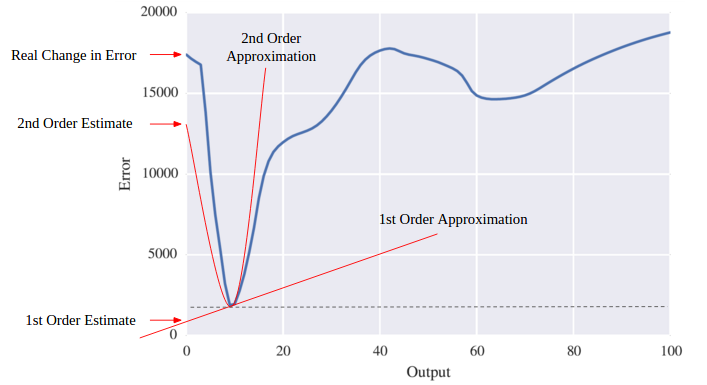
\includegraphics[width=\linewidth]{intuition.png}
  \caption{The intuition behind neuron pruning decision.}
  \label{fig:intuition}
\end{figure}

Figure \ref{fig:intuition} shows a random error function plotted against the output of any given neuron. Note that this figure is for illustration purposes only. The error function is minimized at a particular value of the output as can be seen in the figure. This output is fixed during training as decided by back propagation. Pruning this particular neuron would result in a change in the total error that would be equal to the increase shown in the figure. This neuron is clearly a bad candidate for removal. The straight red line in the figure represents the first-order approximation of the error using Taylor Series as described before while the parabola represents a second-order approximation. It can be clearly seen that the second-order approximation is a much better estimate of the change in error.

We would also like to point out here that it is possible in some cases that there is some thresholding required when trying to approximate the error using the 2nd order Taylor Series expansion. These cases might arise when the parabolic approximation undergoes a steep slope change. To take into account such cases, we employed mean and median thresholding, where any change above a certain threshold was assigned a mean or median value respectively.

Two pruning algorithms are proposed here. They are different in the way the neurons are ranked but both of them use $\Delta E_{k}^2$, the second-order approximation of the error function we got from the Taylor Series, as the basis for the ranking.

The first step in both the algorithms is to  decide a stopping criterion. This can vary depending on the application but some intuitive stopping criteria can be the maximum number of neurons to remove, percentage scaling needed, maximum allowable accuracy drop etc. 

\subsubsection{Algorithm I: Single Overall Ranking}
The complete algorithm is shown in Algorithm \ref{algo1}. The idea here is to generate a single ranked list based on the values of $\Delta E_{k}^2$. This involves a single pass of second-order back-propagation (without weight updates) to collect the gradients for each neuron. The neurons from the formed rank-list (with the least value of $\Delta E_{k}^2$) are then pruned according to the stopping criterion decided.

\begin{algorithm}
 \KwData{optimally trained network, training set}
 \KwResult{A pruned network}
 initialize and define stopping criterion \;
 perform forward propagation over the training set \;
  perform second-order back-propagation without updating weights and collect linear and quadratic gradients \;
  rank the remaining neurons based on $\Delta E_{k}^2$\;
 \While{stopping criterion is not met}{
  remove the last ranked neuron \;
 }
 \caption{Single Overall Ranking}
 \label{algo1}
\end{algorithm}
 
\subsubsection{Algorithm II: Iterative Re-Ranking}

In this greedy variation of the algorithm (Algorithm \ref{algo2}), after each neuron is pruned, the remaining network is made to undergo a single pass of second-order back-propagation (without weight updates) and the rank list is formed again. Hence, each removal involves a new pass through the network. This method is computationally more expensive but takes into account the dependencies the neurons might have with one another which would lead to a change in error contribution every time a dependent neuron is removed. 

\begin{algorithm}
 \KwData{optimally trained network, training set}
 \KwResult{A pruned network}
 initialize and define stopping criterion \;
 \While{stopping criterion is not met}{
  perform forward propagation over the training set \;
  perform second-order back-propagation without updating weights and collect linear and quadratic gradients \;
  rank the remaining neurons based on $\Delta E_{k}^2$  \;
  remove the worst neuron based on the ranking \;
 }
 \caption{Iterative Re-Ranking}
 \label{algo2}
\end{algorithm}
